\defi{10.1} Un polígono $\PP$ es un conjunto finito
$\{\cdots, [V,W],\cdots \}$ de $r$ segmentos llamados lados del polígono. Los extremos de los lados, vértices, forman el conjunto $\{V_1,\cdots,V_r \}$. $\PP$ cumple
\begin{itemizex}
	\item Dos lados de $\PP$ o bien no se cortan o tienen únicamente un extremo común (son lados adyacentes).
	\item Los lados de $\PP$ pueden escribirse como una sucesión finita de vértices $[V_1,V_2],[V_2,V_3],\cdots,[V_r,V_1]$.
\end{itemizex}

\defi{10.4} Une \textbf{diagonal} es un segmento cuyos extremos son dos vértices que no pertenecen al mismo lado.

\defi{10.6} Sea $V$ un vértice de $\PP$ y sean $[V,W_1]$ y $[V,W_2]$ dos lados. El ángulo con vértice $V$ y semirrectas que contienen a ambos lados forman el ángulo $\angle V$ de $\PP$.

\defi{10.8} Un polígono es \textbf{convexo} si toda recta que no contiene a ninguno de los lados del polígono corta a lo sumo en dos lados de éste.

 \tma{10.10} Un polígono $\PP$ es convexo sii para todo lado $[V,W]$ de $\PP$ los vértices de $\PP$ distintos de $V$ y $W$ están todos en el mismo de los dos semiplanos determinados por $r_{VW}$.
 
 \defi{10.11} Un punto $P$ está en el \textbf{interior} de un polígono convexo $\PP$ si cualquier recta que pase por $P$ corta a los lados del polígono en dos puntos. Si $P$ no está ni en el interior ni en los lados del polígono, entonces está en el exterior. 
 
 \obs{10.12} Un punto $P$ está en el interior de un polígono $\PP$ si existe una recta $r$ que pasa por $P$ de modo que si $\overline{s}$ es una de las semirrectas, $\overline{s}$ corta a $\PP$ en un número $n$ impar de puntos que no son vértices.
 
 \defi{10.13} Un polígono convexo es \textbf{regular} si todos sus lados y ángulos son congruentes.
 
 \lema{10.14} Sean $r$ y $s$ rectas que al cortarse forman un ángulo $\pi/n$. Sean $\sigma_r$ y $\sigma_s$. Si $V$ es un punto en $r$, definimos los puntos $V_{i+1} = (\sigma_s \circ \sigma_r)^i(V), \quad i=1,\cdots, n-1$, es decir, las imágenes de $V$ por rotaciones. Entonces, si $V_1 = V$, el polígono
 $$\PP= \{[V_1,V_2],\cdots,[V_{n-1},V_n],[V_n,V_1]  \}$$
 es regular.
 
 \tma{10.15} Sea $n$ entero mayor que 2. Sea $[V,W]$ un segmento del plano, y $H$ uno de los semiplanos determinados por $r_{VW}$. Existe un polígono regular de $n$ lados contenido en $H \cup r_{VW}$ y uno de los lados es $[V,W]$. \cor{10.17} En estas condiciones $\PP$ es único.
 
 \tma{10.16/10.19} Sea $\PP$ regular con $n$ vértices. $\PP$ admite $n$ reflexiones distintas, que son simetrías de $\PP$. También existe una rotación con ángulo $2\pi/n$ que es simetría de $\PP$. Análogamente, si $\PP$ es convexo con $n$ vértices y tiene como simetría una rotación $2\pi/n$, entonces es regular.
 
\cor{10.18} Todo $\PP$ regular permite una circunferencia $\C$ que pase por todos sus vértices. Entonces $\PP$ está \textbf{inscrito} en $\C$.
\vspace{-2em}
\subsection*{Construcciones con regla y compás}
\tma{10.24}/\defi{10.26} Dados dos puntos $A$ y $B$ se puede construir un punto $C \in [A,B]$ con regla y compás de modo que $AB\cdot BC = AC^2$. $C$ divide en razón áurea, $\frac{AB}{AC} = \frac{1+\sqrt{5}}{2}$.
	\begin{figure}[H]
	\centering
	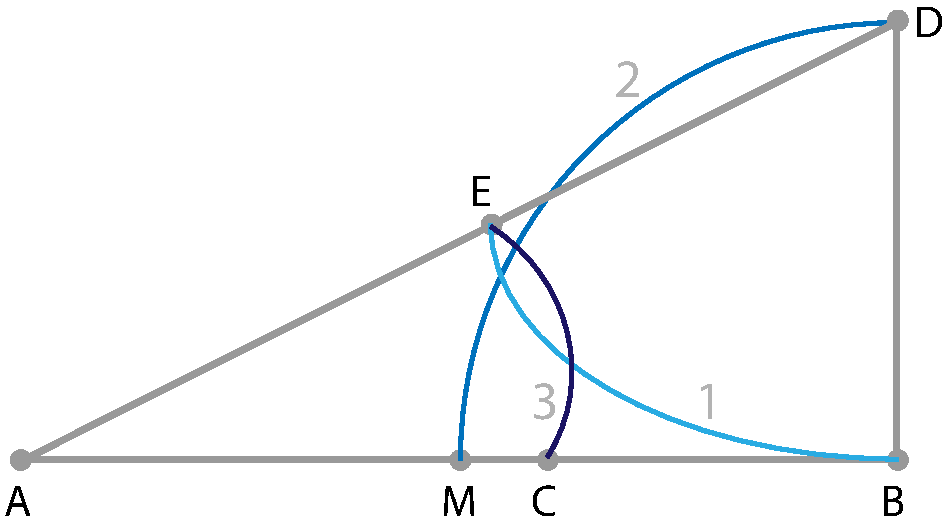
\includegraphics[width=7.5cm]{figuras/10-24.pdf}
	\vspace{-1em}
\end{figure}
\obligatorio\dem{La construcción está contenida en la figura. Se puede demostrar la igualdad por el \tma{de Pitágoras}, escribiendo todo en función de $AB$:
$$AB^2 + \left(\frac{1}{2}AB\right)^2 = AD^2 = (AC + \frac{1}{2}AB)^2$$
$$AB^2 + \cancel{\frac{1}{4}AB^2} = AC^2 + \cancel{\frac{1}{4}AB^2} + ACAB = AC^2 + (AB-BC)AB$$
$$\cancel{AB^2}=AC^2+\cancel{AB^2}-ABBC\iff AC^2 = AB\cdot BC$$
}

\tma{10.27, 10.28} Sea $\triangle ABC$ un triángulo isósceles tal que $AB = AC$ y $\measuredangle B = \measuredangle C = 2\measuredangle A$. Entonces $\frac{AB}{BC}$ es la razón áurea. Además, este triángulo puede construirse con regla y compás.

\obs{10.29}/\cor{10.30} El ángulo $\measuredangle A$ del triángulo áureo es $\pi/5$. Por tanto, se puede construir un pentágono regular con lados congruentes a $[A,B]$.

\tma{10.31} Un polígono regular de $n$ lados se puede construir con regla y compás sii la factorización de $n$ en números primos tiene la forma $n = 2^kp_1p_2\cdots p_m$, con $p_i$ de la forma $2^{2^s}+1$, y son primos distintos. Así, los lados polígonos construibles son $3,4,5,6,8,10,12,15,16,17, \cdots$.



 

